\documentclass[12pt,onecolumn]{article}
\usepackage[utf8]{inputenc} % UTF8 input encoding
\usepackage[T2A]{fontenc}   % T2A font encoding for Cyrillic script
\usepackage[russian]{babel} % Russian language support
\usepackage{listings}
\usepackage{float}
\usepackage{mathtools}
\everymath{\displaystyle}
\usepackage{listings} 
\usepackage[usenames]{color}
\usepackage{hyperref}
\usepackage{geometry}
\usepackage{verbatim}
\newcommand{\nparagraph}[1]{\paragraph{#1}\mbox{}\\}
\geometry{
  a4paper,
  top=20mm, 
  right=20mm, 
  bottom=20mm, 
  left=25mm
}

\begin{document}
\setcounter{tocdepth}{4}
\begin{center}
    Федеральное государственное автономное образовательное учреждение высшего образования "Национальный Исследовательский Университет ИТМО"\\ 
    Мегафакультет Компьютерных Технологий и Управления\\
    Факультет Программной Инженерии и Компьютерной Техники \\
    
\includegraphics[scale=0.3]{image/itmo.jpg} % нужно закинуть картинку логтипа в папку с отчетом
\end{center}
\vspace{1cm}


\begin{center}
    \large \textbf{Вариант №2}\\
    \textbf{Лабораторная работа 1}\\
    по дисциплине\\
    \textbf{'Функциональная схемотехника'}
\end{center}

\vspace{2cm}

\begin{flushright}
  Выполнил Студент  группы P33102\\
  \textbf{Лапин Алексей Александрович}\\
  Преподаватель: \\
  \textbf{Васильев С.Е.}\\
\end{flushright}

\vspace{9cm}
\begin{center}
    г. Санкт-Петербург\\
    2024г.
\end{center}
\pagestyle{empty}

\newpage
\tableofcontents
\newpage
\pagestyle{plain}
\section{Цели работы:}
\begin{enumerate}
    \item Получить базовые знания о принципах построения цифровых интегральных схем с использованием технологии КМОП.
    \item Познакомиться с технологией SPICE-моделирования схем на транзисторах.
    \item Получить навыки описания схем базовых операционных элементов (БОЭ) комбинационного типа на вентильном уровне с использованием языка описания аппаратуры Verilog HDL.
\end{enumerate}
\section{Задание}
Лабораторная работа состоит из двух частей.

Первая часть посвящена проектированию цифровых вентилей на полевых транзисторах, построению схем на базе вентилей и знакомству с технологией SPICEмоделирования. Первая часть работы выполняется в программном пакете LTspice. При построении схем вентилей необходимо использовать КМОП-транзисторы с параметрами из файла, предоставленного преподавателем (см. раздел «Основы работы в среде LTspice»).

Вторая часть посвящена знакомству с языком описания аппаратуры Verilog HDL, изучению особенностей его использования для описания схем на вентильном уровне и приобретению навыков тестирования таких схем. Вторая часть работы выполняется с использованием Vivado Simulator, входящего в пакет Vivado Design Suite (см. раздел «Основы работы в среде Vivado Design Suite»).

\textbf{Вариант}: 2

\textbf{Логический базис}: NAND

\textbf{БОЭ}: Полный четырехразрядный компаратор

\section{Отчет о выполнении заданий части 1:}
\subsection{Схема разработанного вентиля NAND}
\begin{figure}[H]
    \centering
    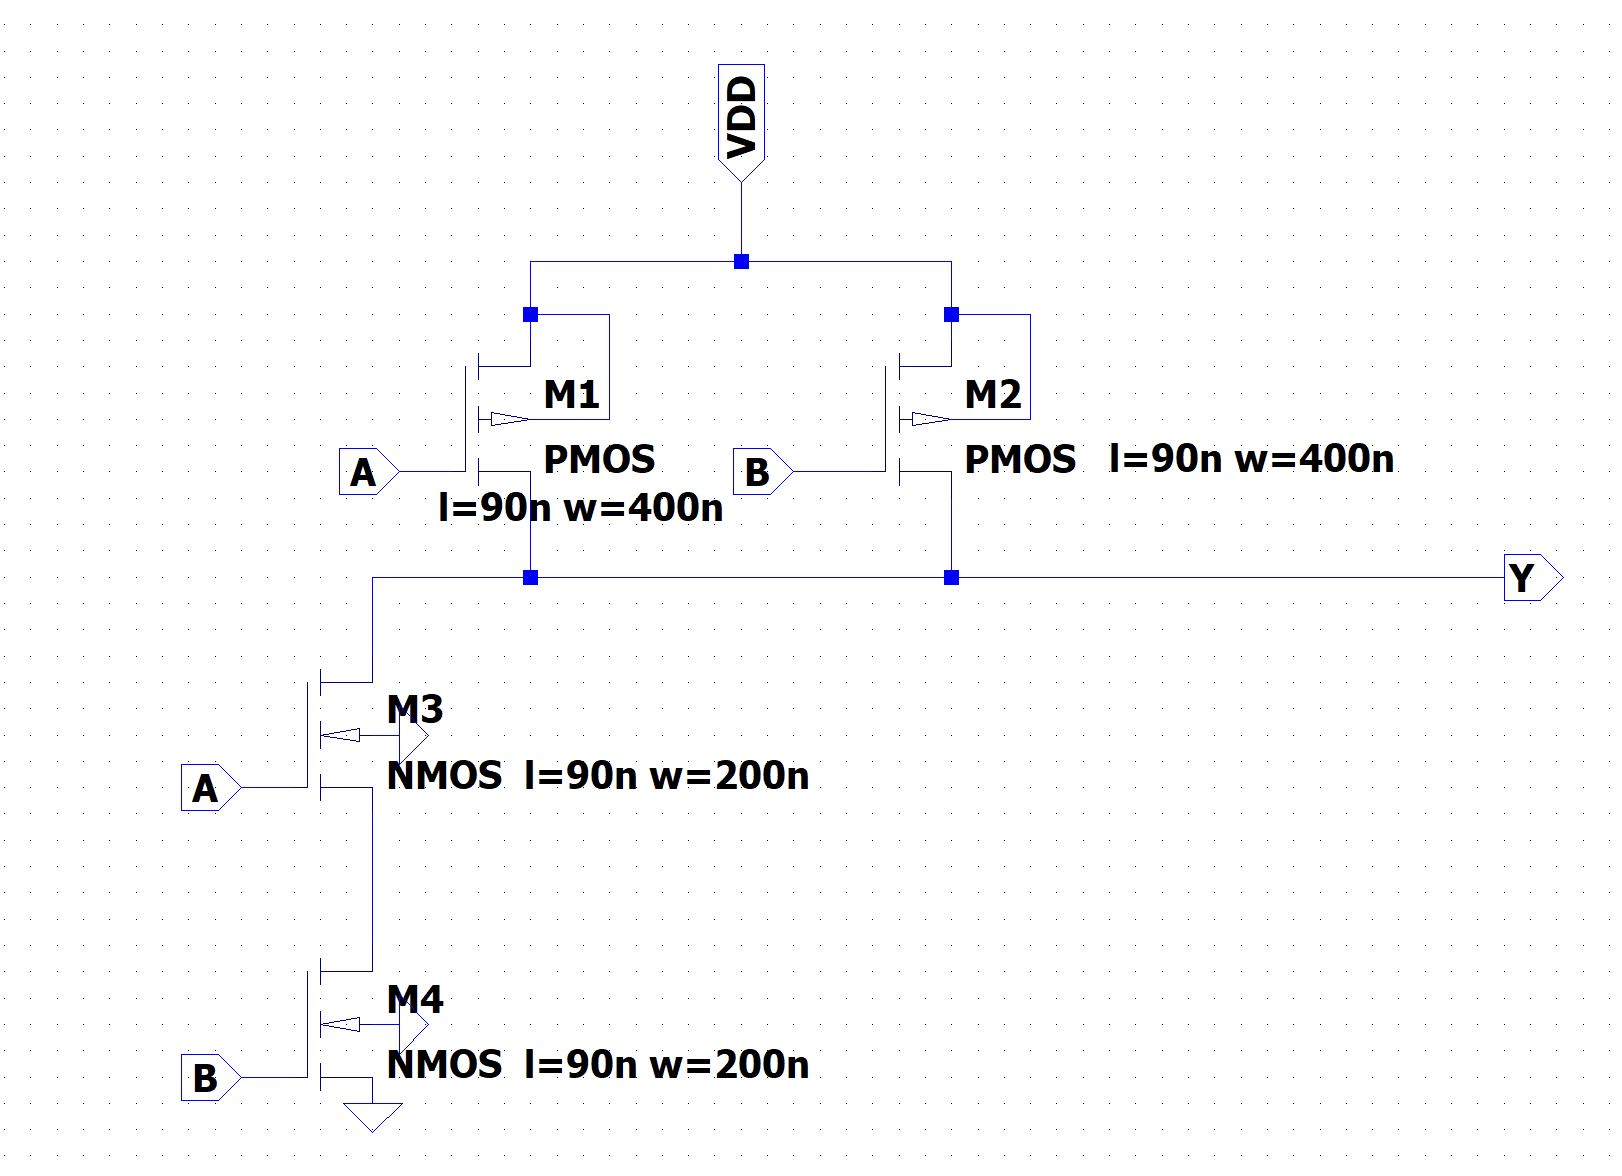
\includegraphics[scale=0.5]{image/ventil.png}
    \caption{Схема разработанного вентиля NAND}
\end{figure}
\subsection{Символ вентиля и схема тестирования}
\begin{figure}[H]
    \centering
    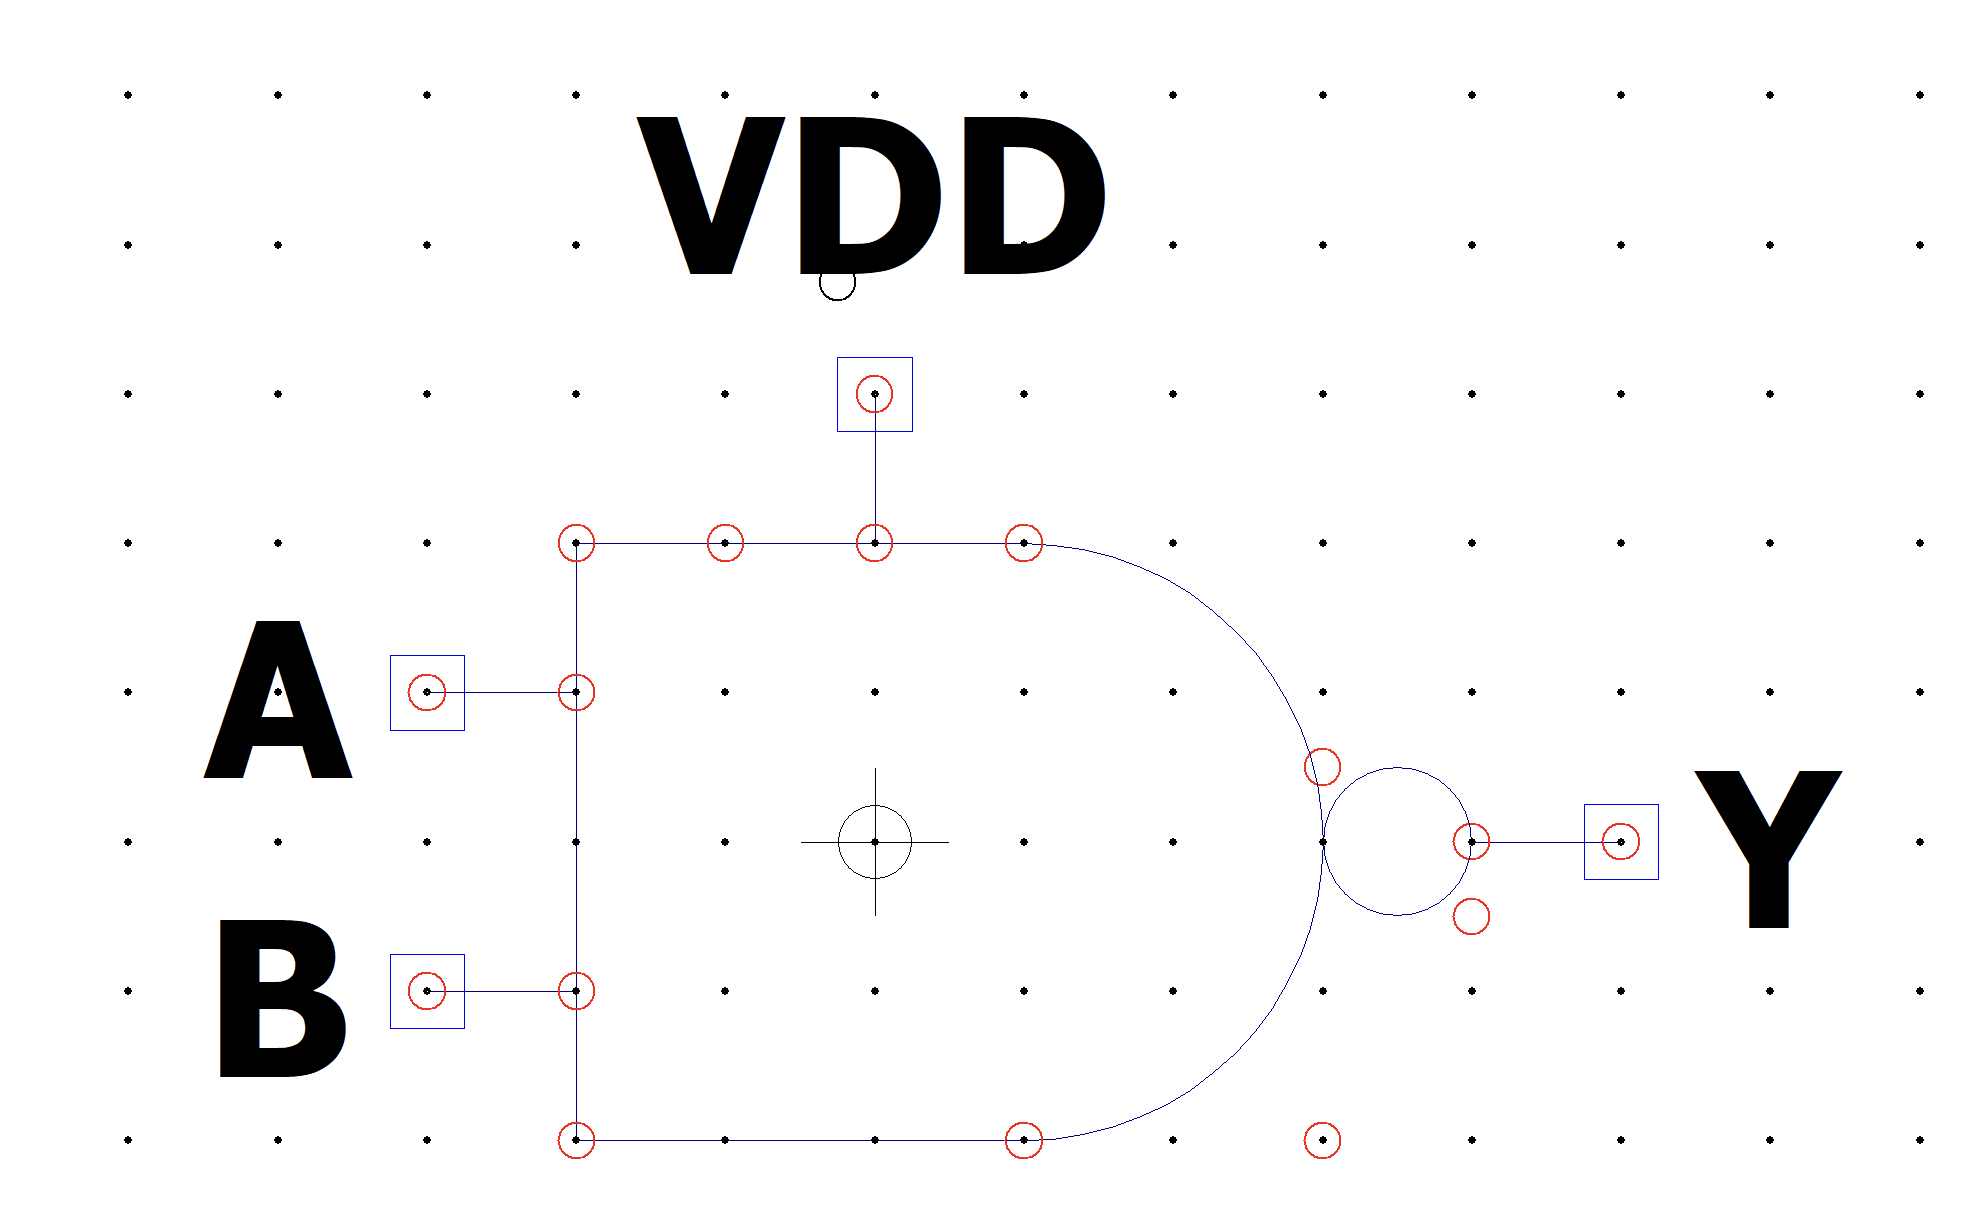
\includegraphics[scale=0.2]{image/symbol.png}
    \caption{Символ вентиля}
\end{figure}
\begin{figure}[H]
    \centering
    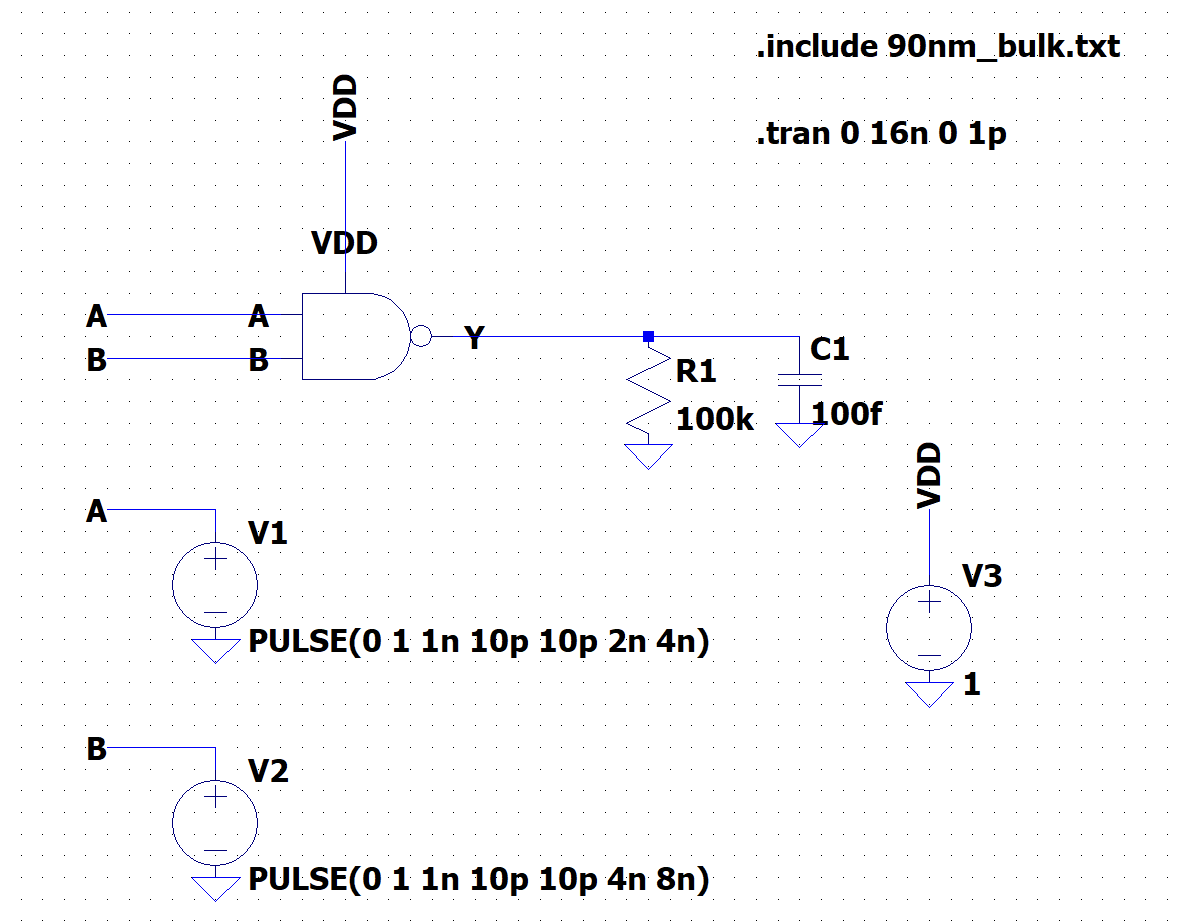
\includegraphics[width=\textwidth]{image/test-circuit.png}
    \caption{Схема тестирования}
\end{figure}
\subsection{Временная диаграмма процесса тестирования вентиля}
\begin{figure}[H]
    \centering
    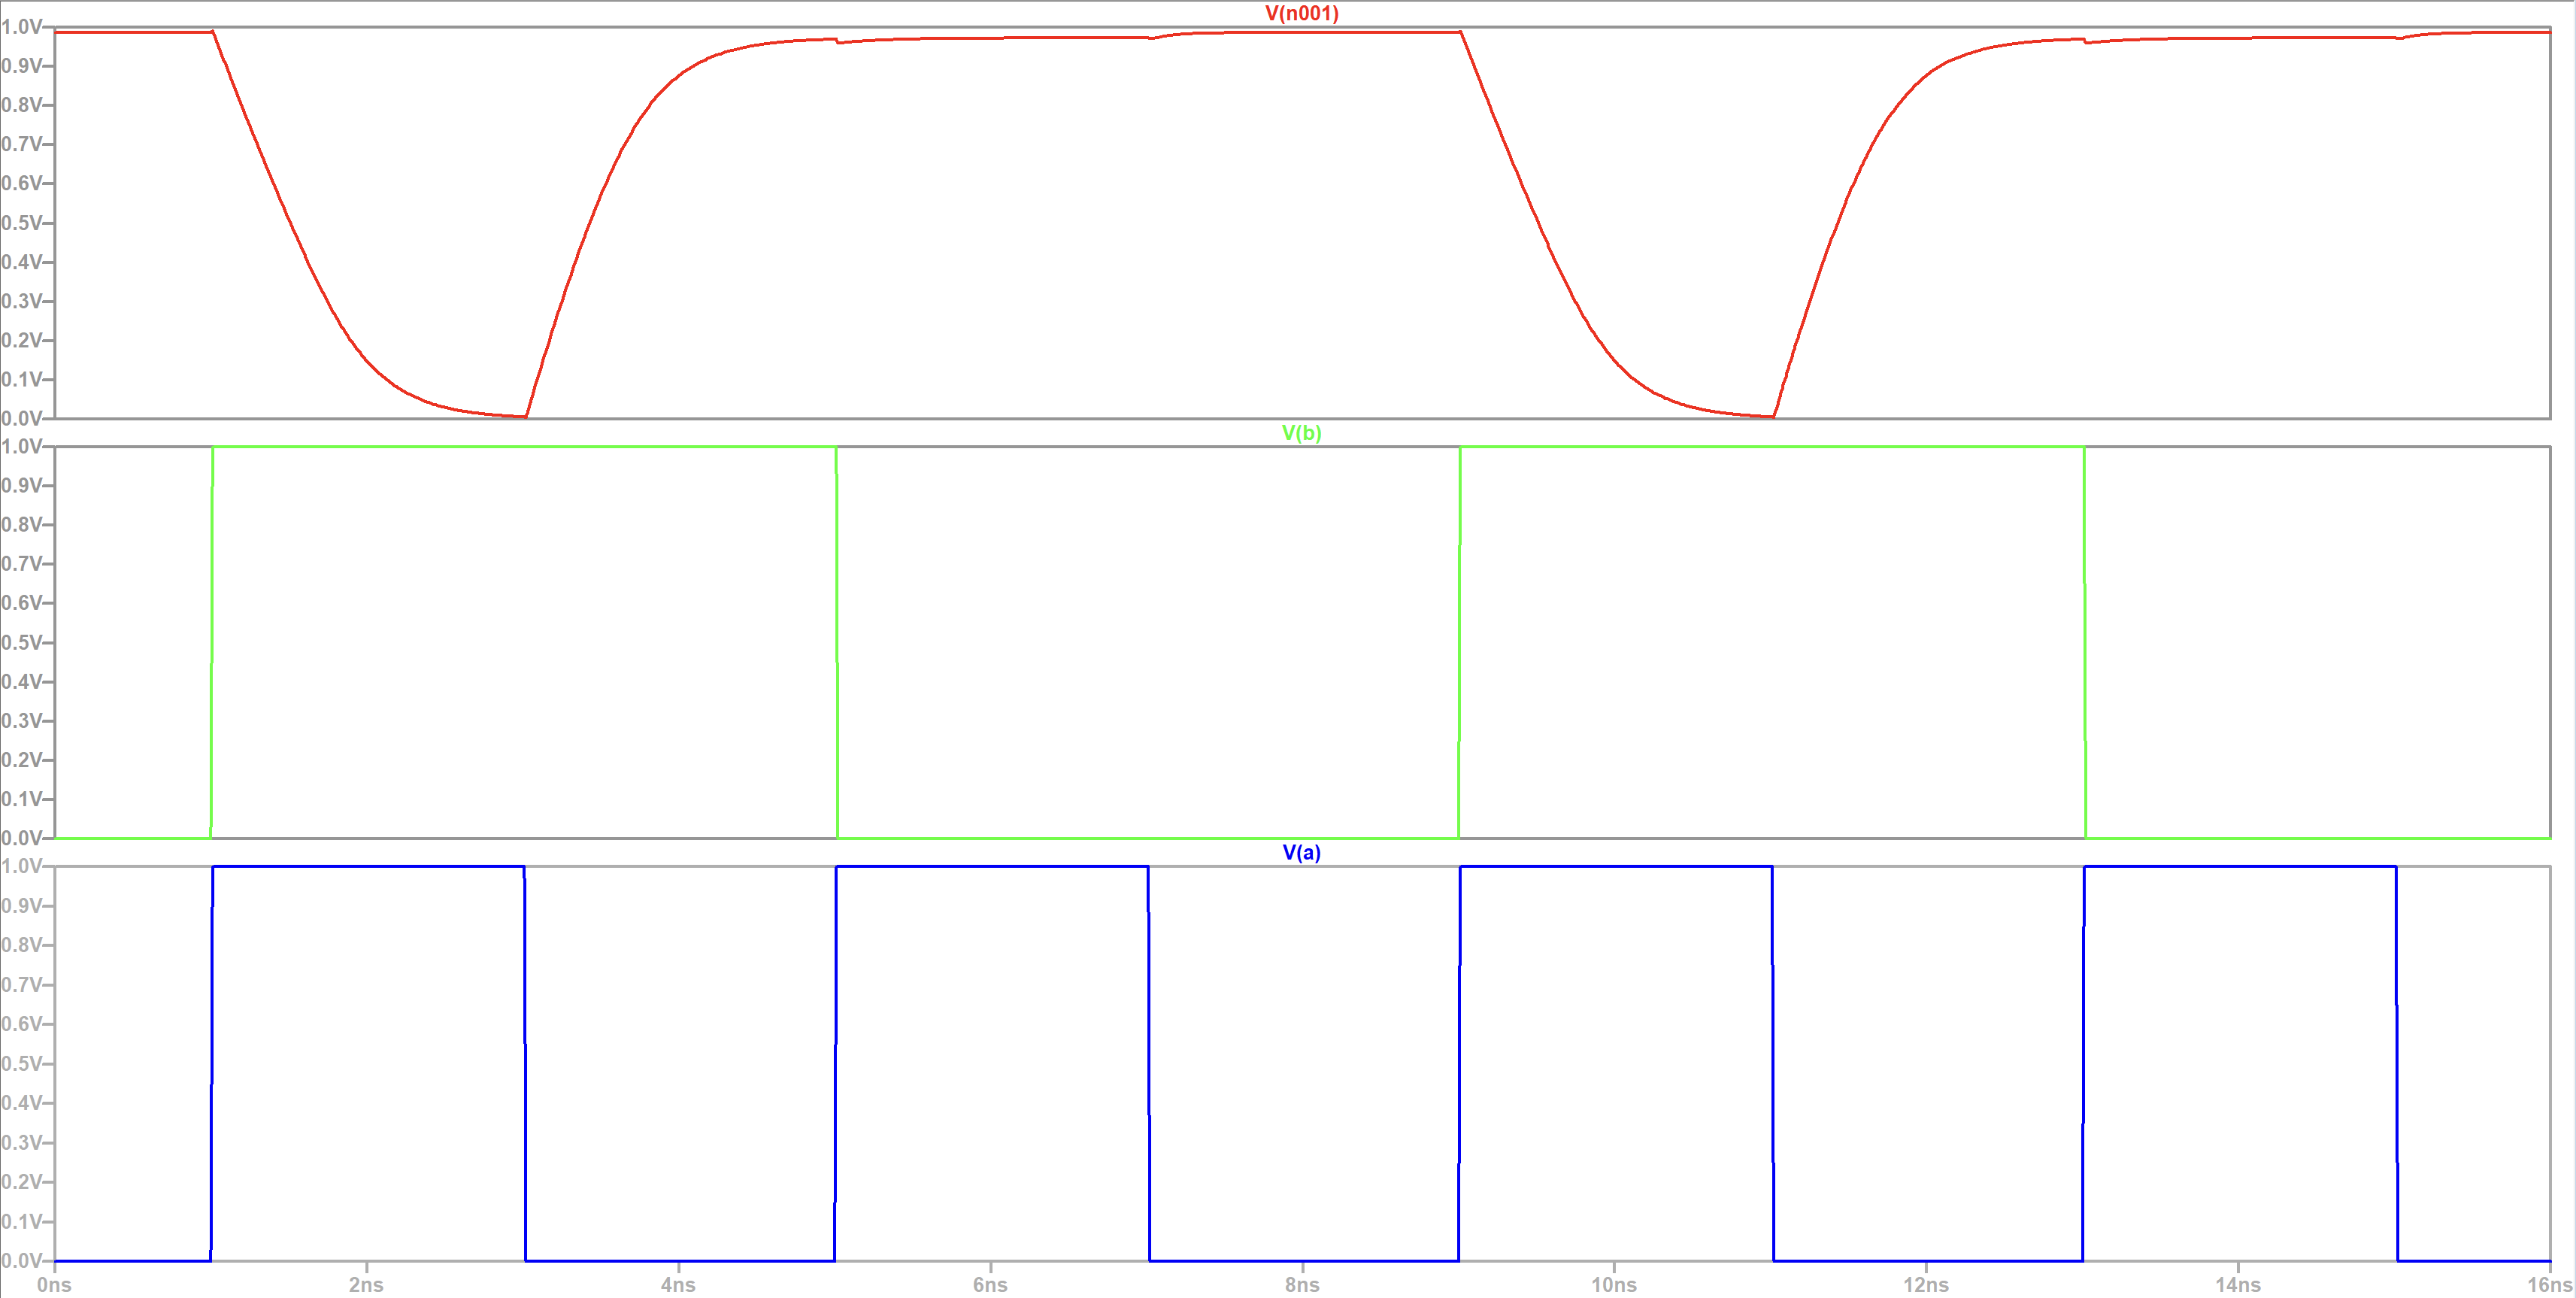
\includegraphics[width=\textwidth]{image/time-diagram.png}
    \caption{Временная диаграмма процесса тестирования вентиля}
\end{figure}
\subsection{Результат измерения задержки распространения сигнала через вентиль}
Задержка распространения - максимальное время от начала изменения входа до момента,
когда все выходы достигнут установившихся значений. Измеряется она между точками
перехода входным и выходным сигналом уровня 50\%.
\begin{figure}[H]
    \centering
    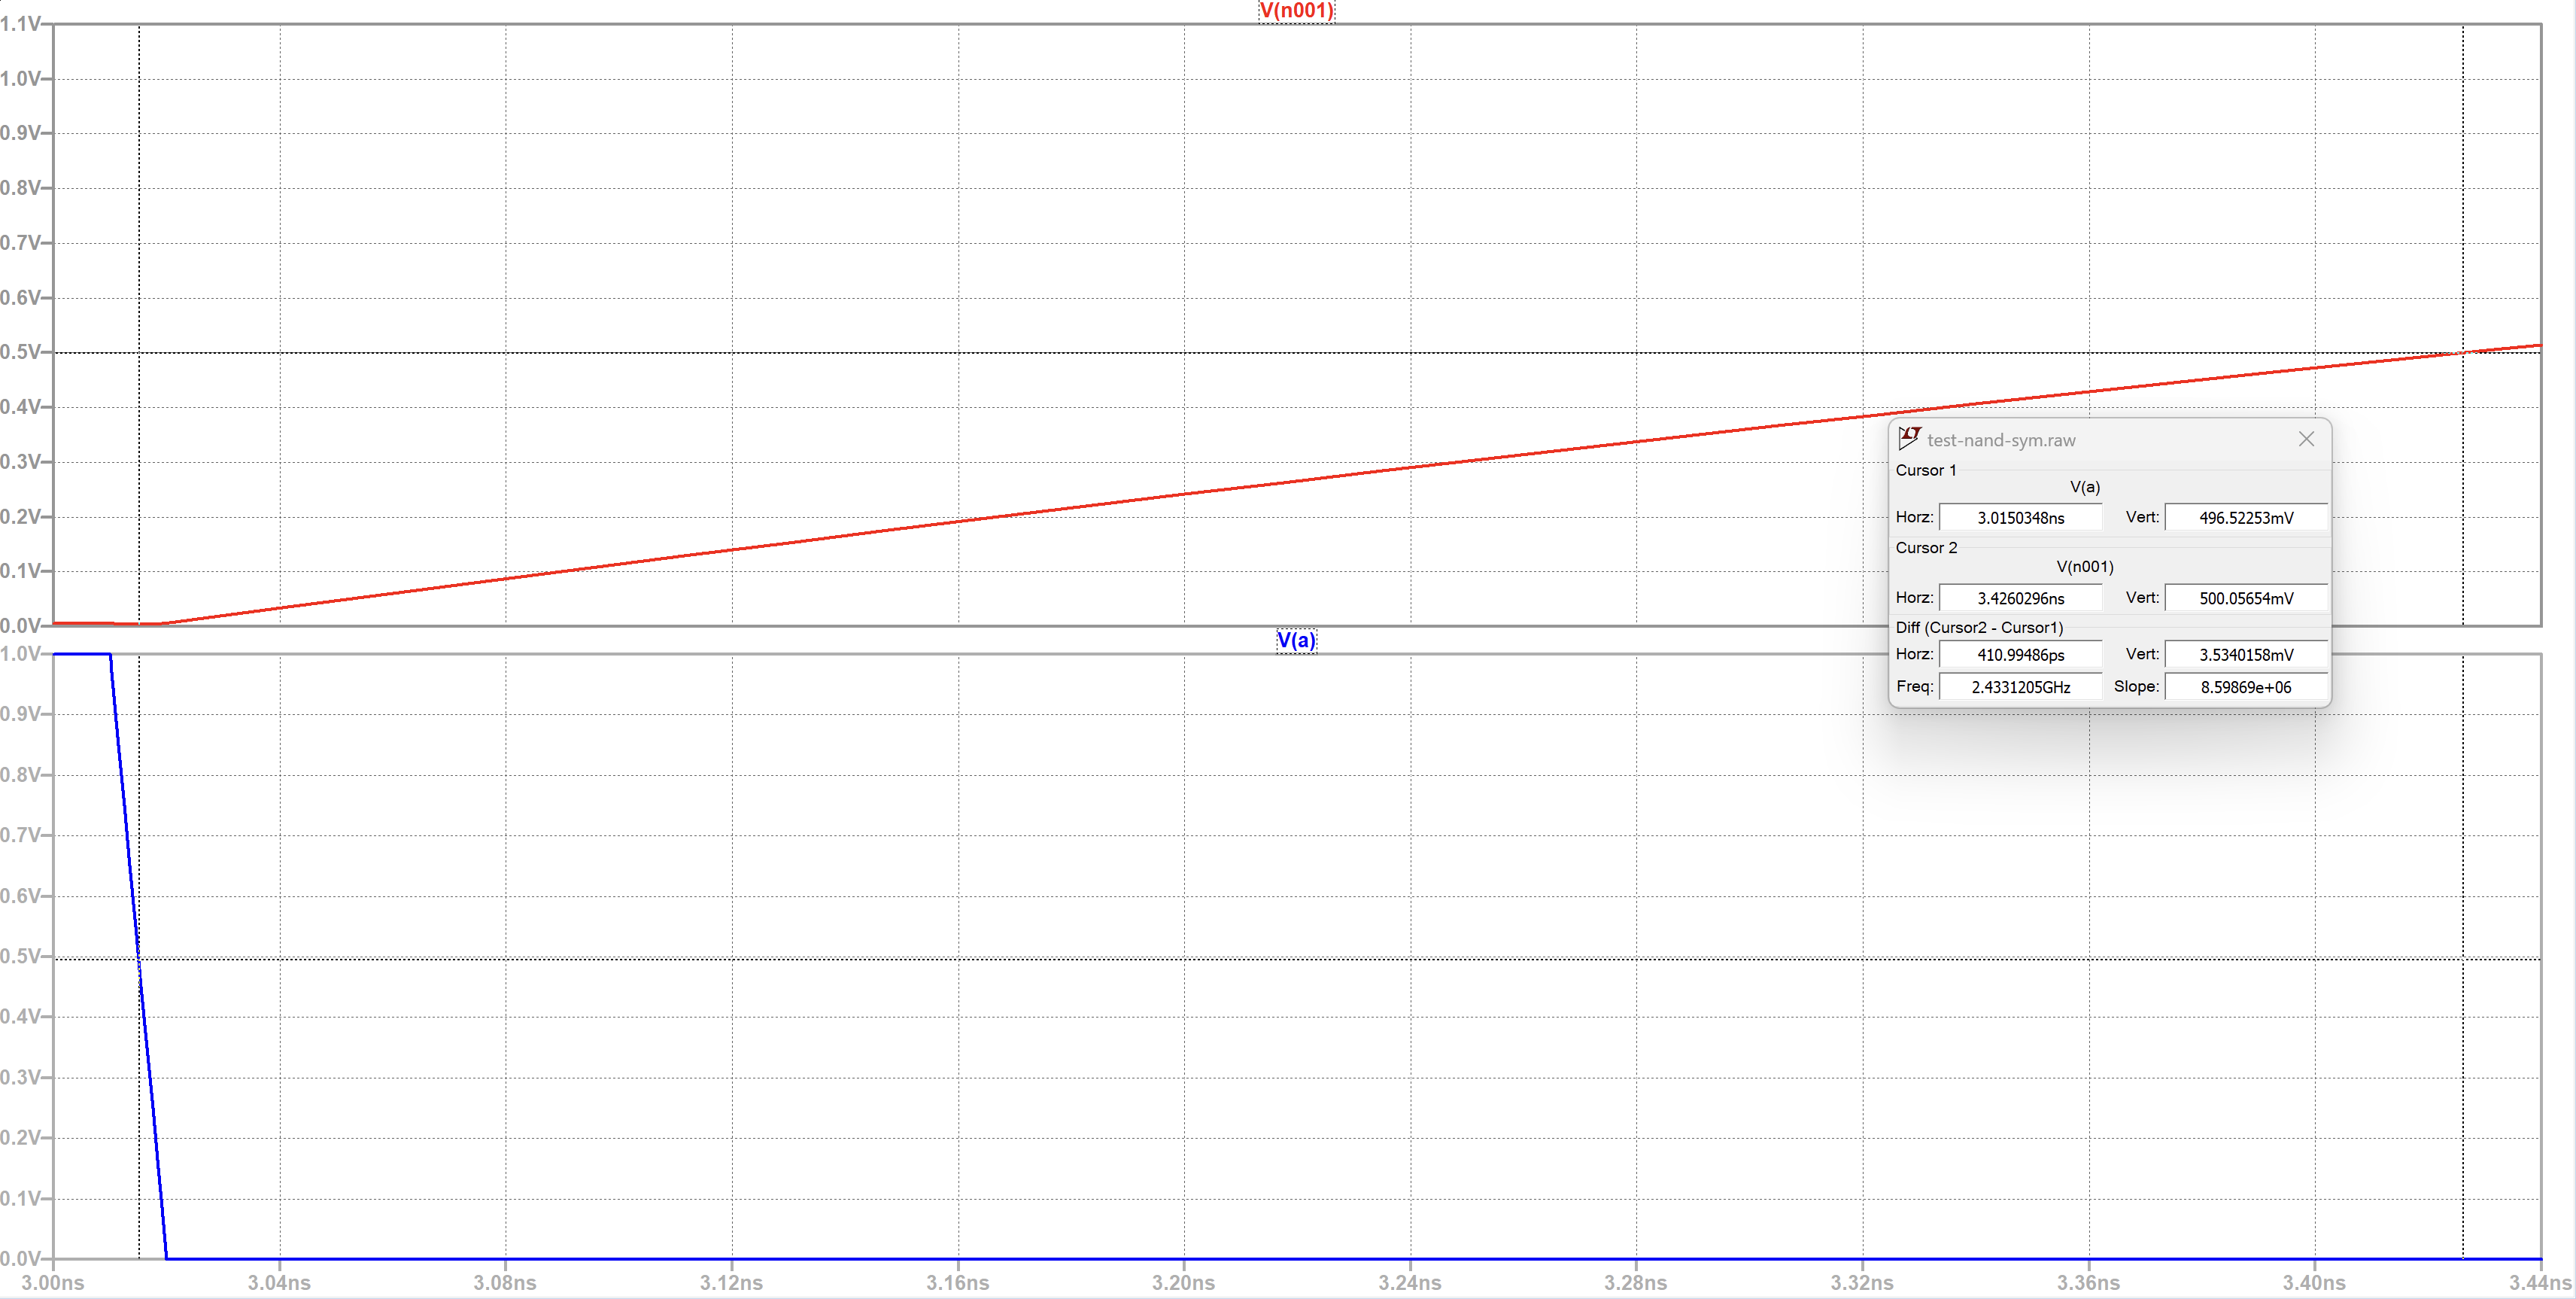
\includegraphics[width=\textwidth]{image/delay0-1.png}
    \caption{Подсчет задержки распространения сигнала для 0-1 на выходе}
\end{figure}
\begin{figure}[H]
    \centering
    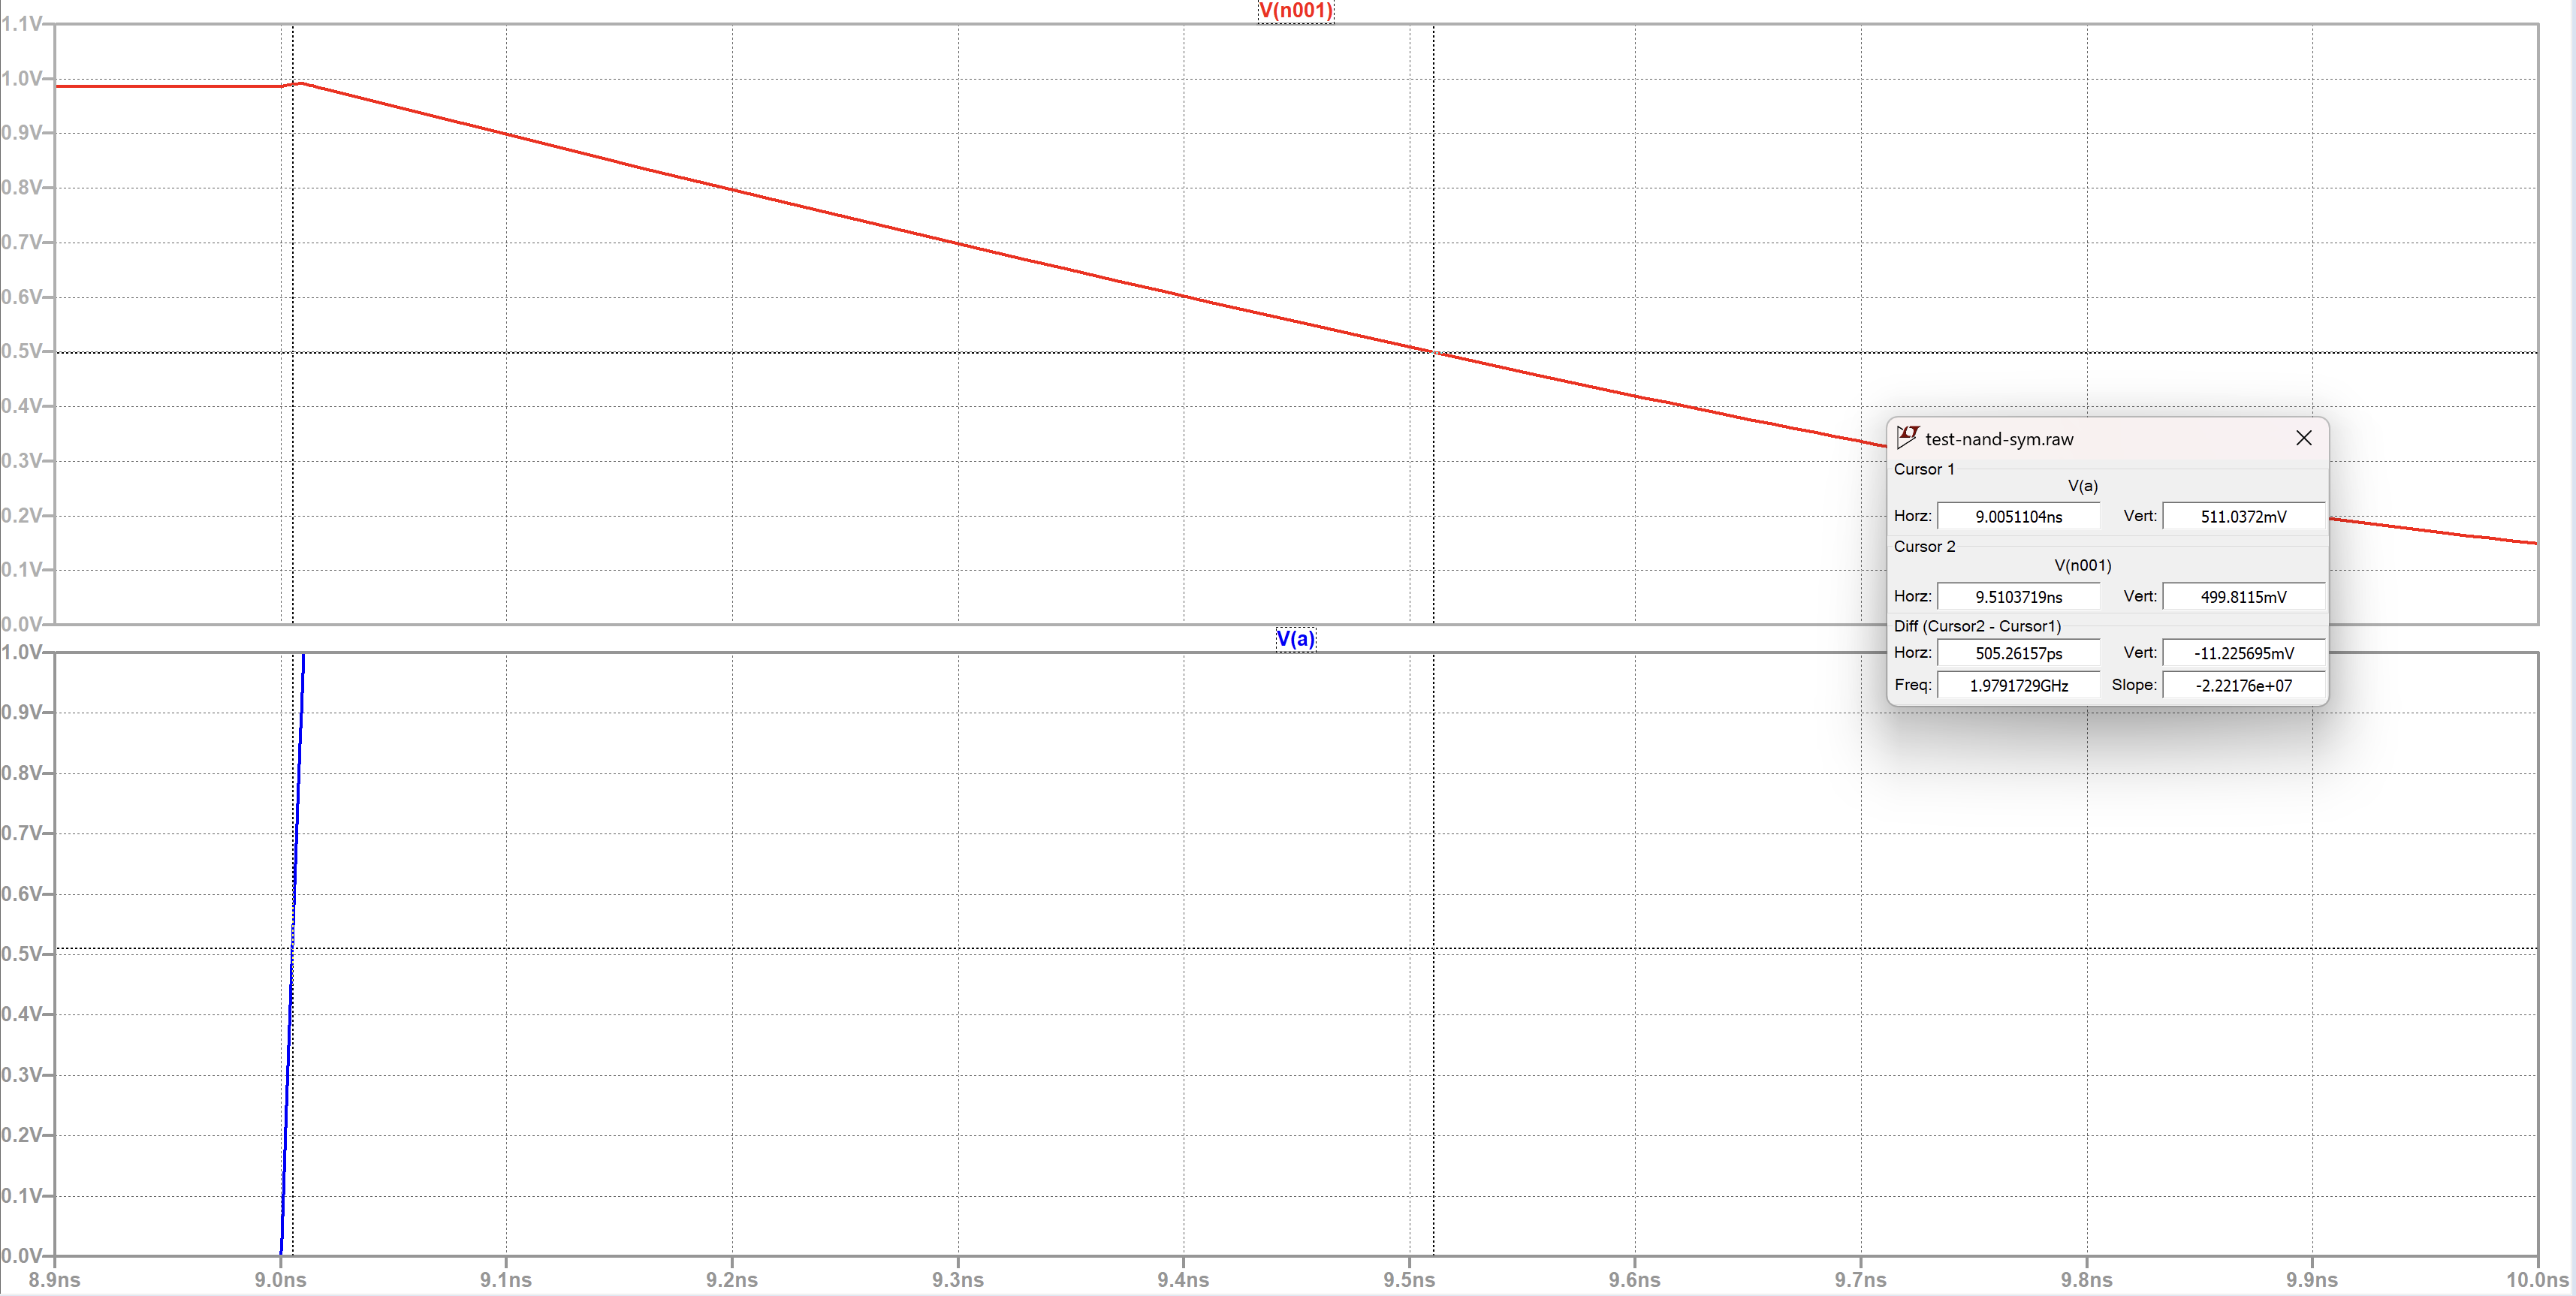
\includegraphics[width=\textwidth]{image/delay1-0.png}
    \caption{Подсчет задержки распространения сигнала для 1-0 на выходе}
\end{figure}
$$
    t_{pd} = t_2 - t_1 = 3.426 - 3.015 = 0.411 \text{нс} - \text{задержка распространения сигнала для 0-1 на выходе}
$$
$$
    t_{pd} = t_2 - t_1 = 9.510 - 9.005 = 0.505 \text{нс} - \text{задержка распространения сигнала для 1-0 на выходе}
$$
\subsection{Максимальная частота работы вентиля}
Высчитывается как время спада(фронта) от 0.1 до 0.9 (0.9 до 0.1) уровня на выходе вентиля, и от этого времени высчитывается частота:
\begin{figure}
    \centering
    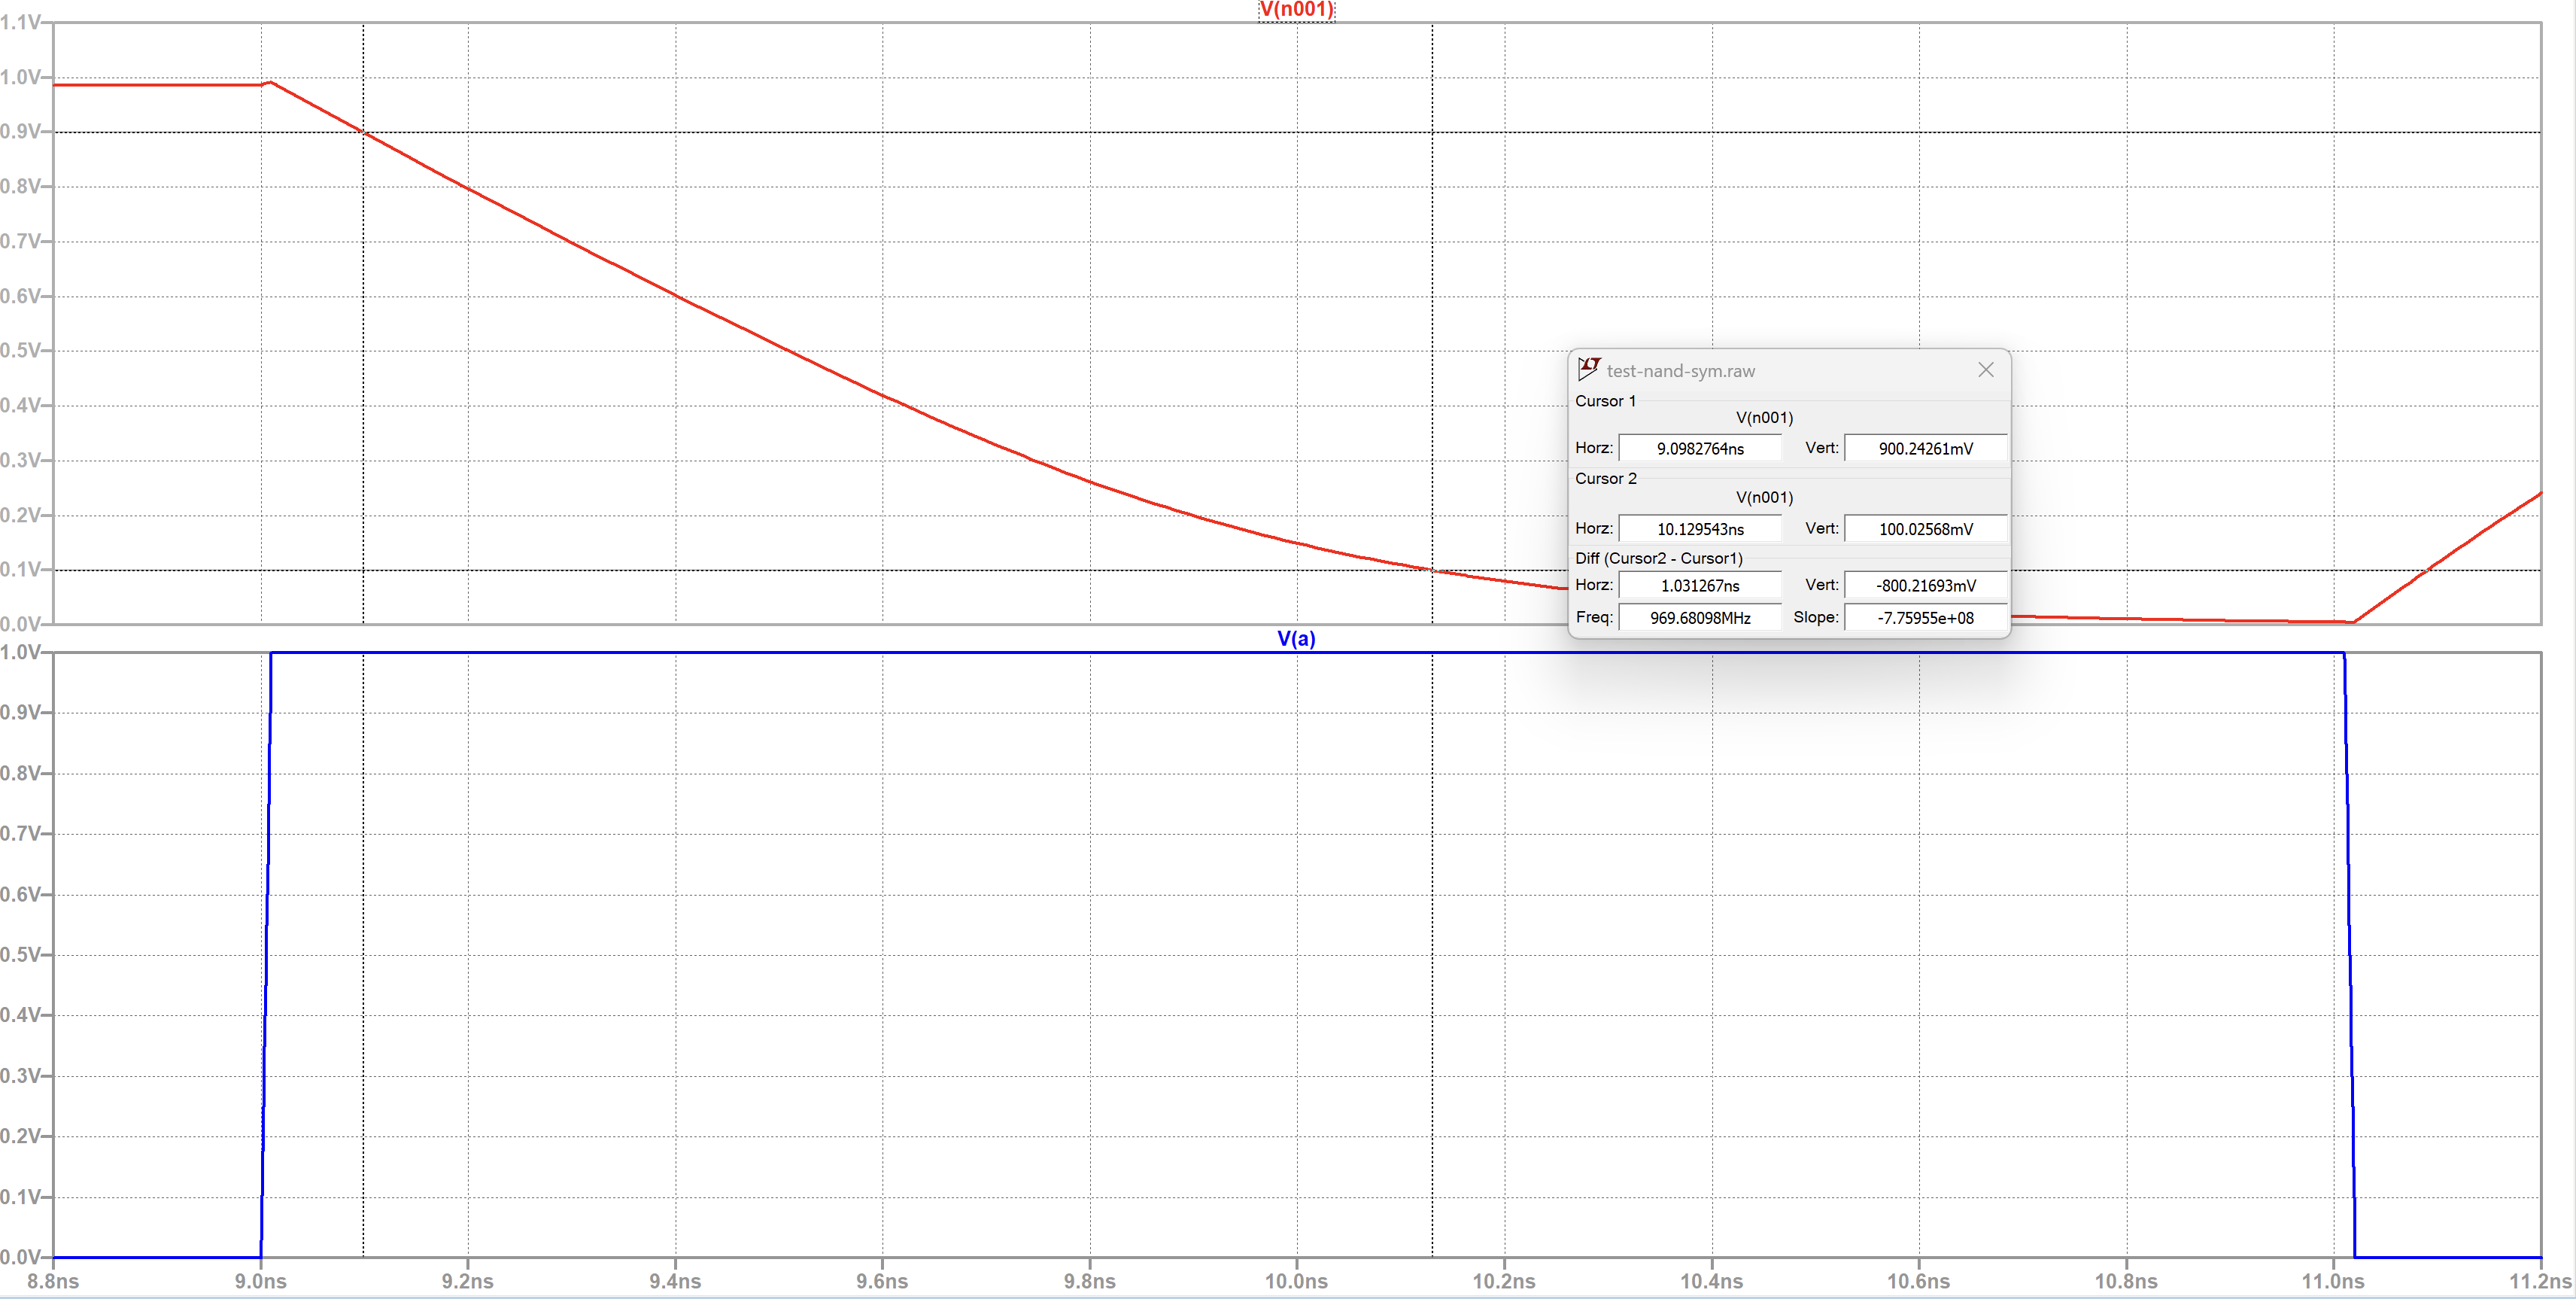
\includegraphics[width=\textwidth]{image/frequency10.png}
    \caption{Время спада от 0.9 до 0.1}
\end{figure}
\begin{figure}[H]
    \centering
    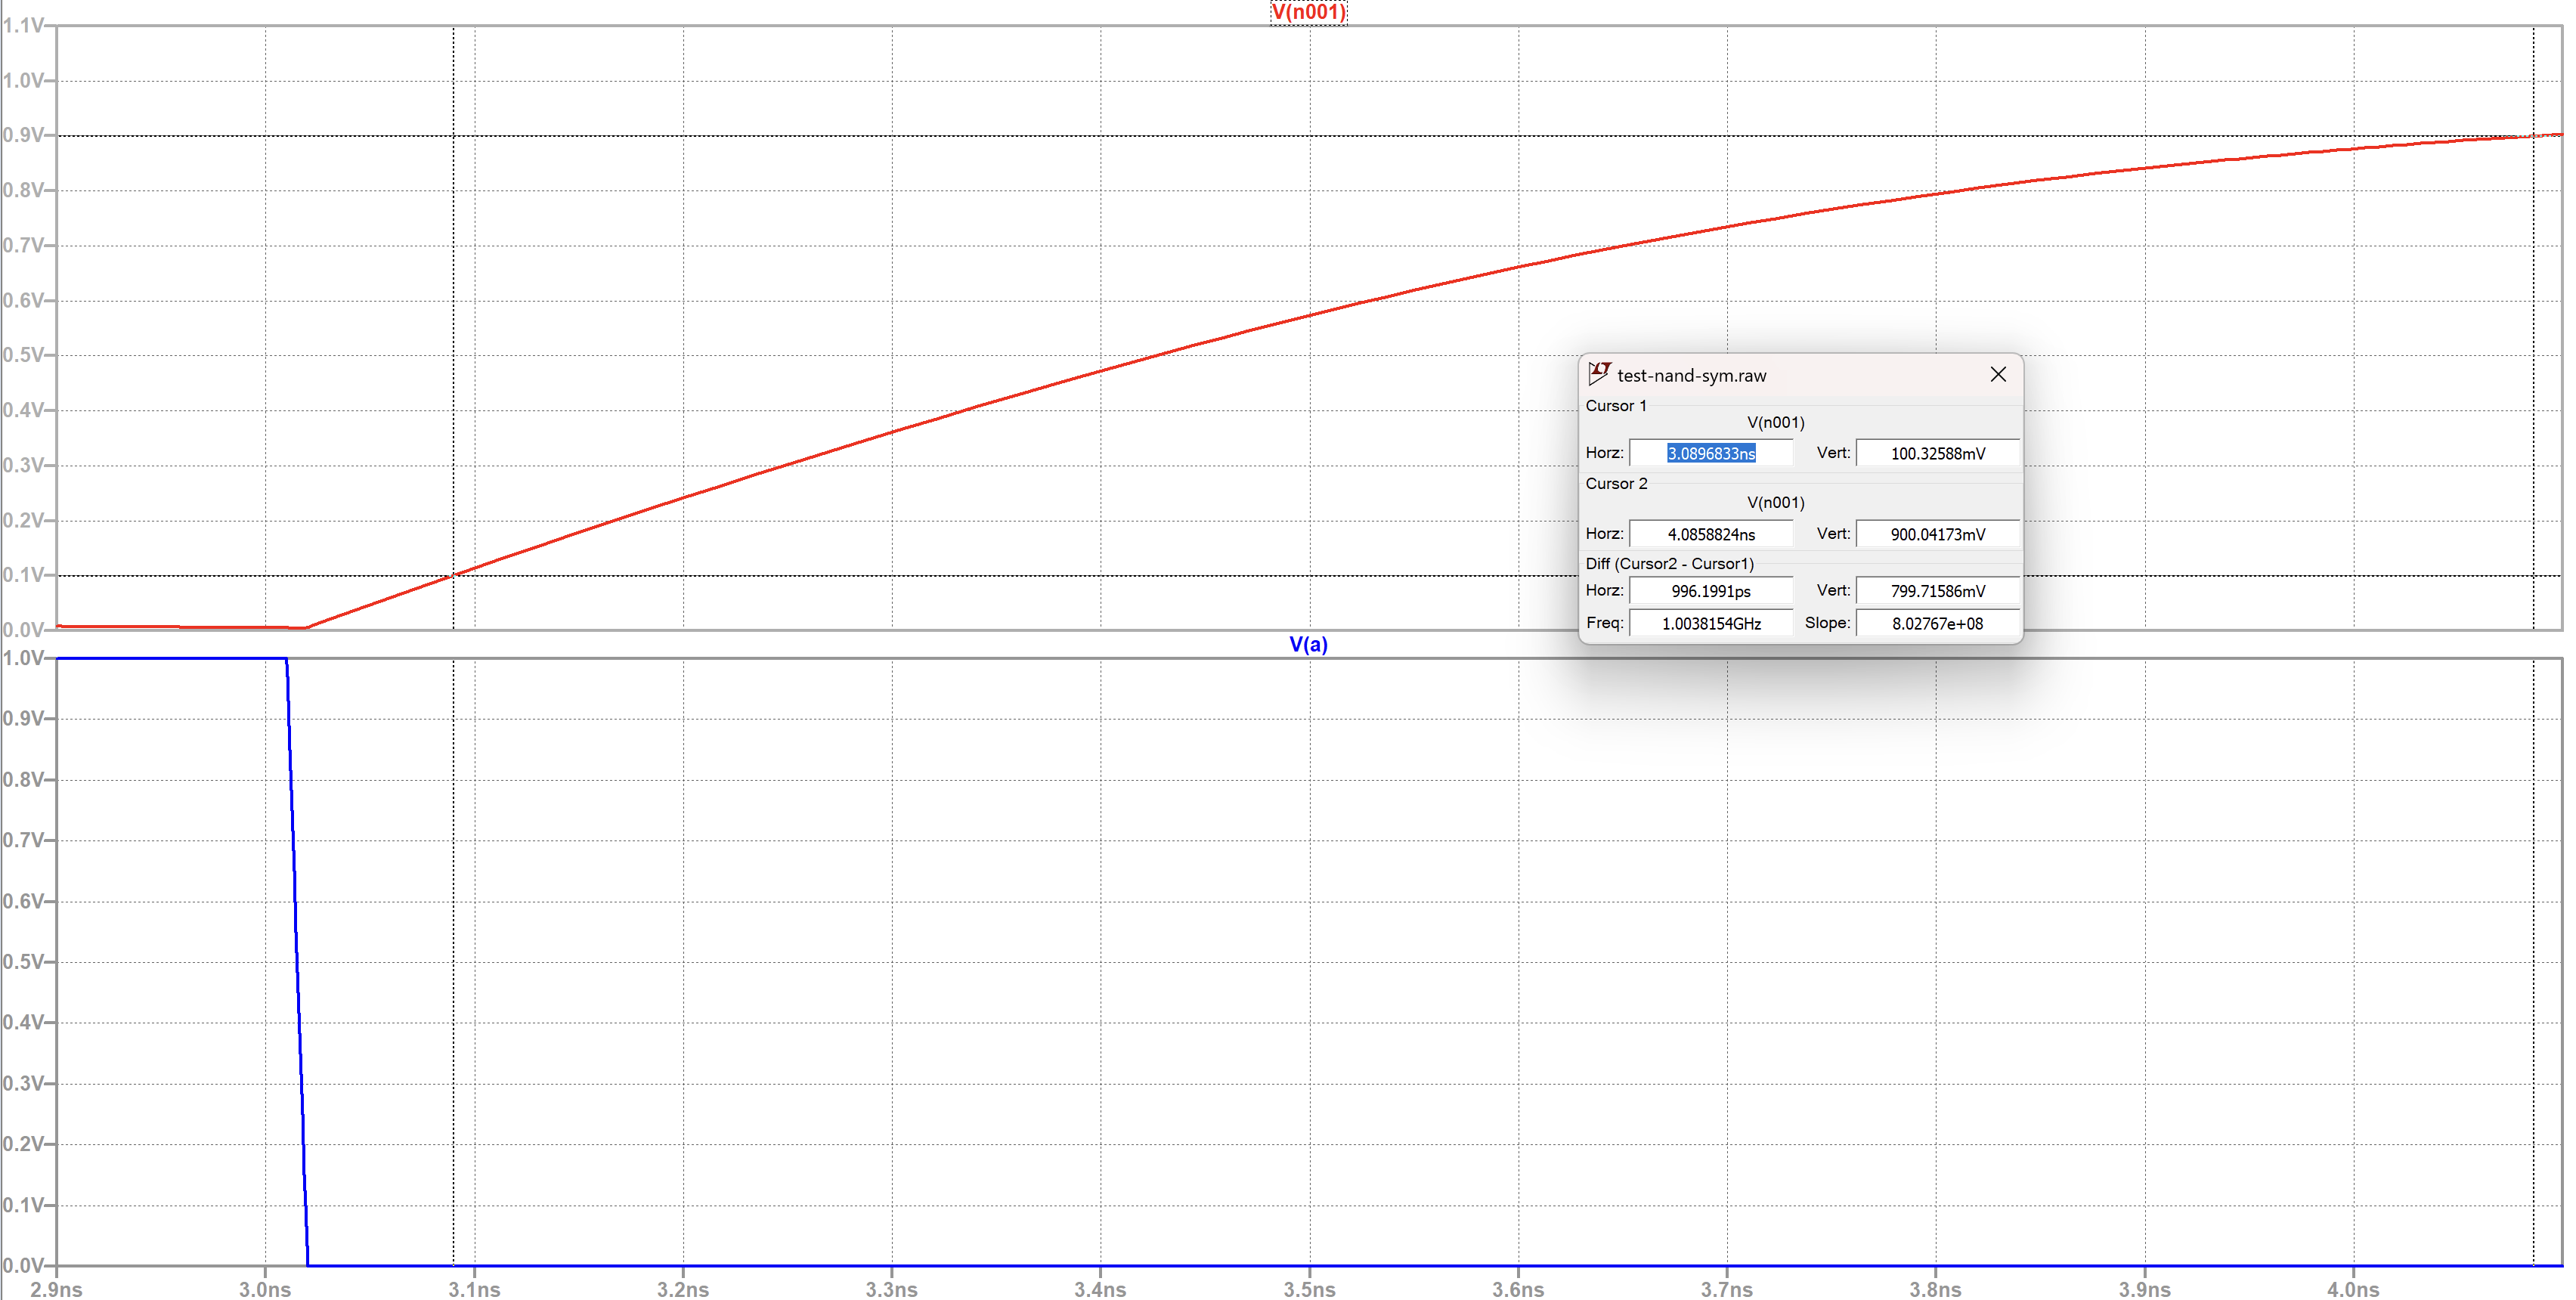
\includegraphics[width=\textwidth]{image/frequency01.png}
    \caption{Время фронта от 0.1 до 0.9}
\end{figure}
$$
    t_{10} = 9.098 - 10.130 = 1.031 \text{нс} - \text{для спада}
$$
$$t_{01} = 4.086 - 3.089 = 0.996 \text{нс} - \text{для фронта}$$
Тогда частота спада/фронта:
$$
    \nu_{\text{спада}} = \frac{1}{t_{10}} = \frac{1}{1.031} = 0.970 \text{ГГц}
$$
$$
    \nu_{\text{фронта}} = \frac{1}{t_{01}} = \frac{1}{0.996} = 1.004 \text{ГГц}
$$
Тогда максимальная частота работы вентиля:
$$
\nu_{\max} = \min(\nu_{\text{спада}}, \nu_{\text{фронта}}) = \min(0.970, 1.004) = 0.970 \text{ГГц}
$$

\end{document}